\documentclass[tikz]{standalone}

\usepackage{amsmath}
\usepackage{lmodern}
\usepackage{pgfplots}
%\usepackage{physics}

\let\Re\undefined
\let\Im\undefined
\DeclareMathOperator{\Re}{\operatorname{Re}}
\DeclareMathOperator{\Im}{\operatorname{Im}}

\usetikzlibrary{arrows.meta,decorations.markings}
%\pgfplotsset{compat=1.17}

\begin{document}
	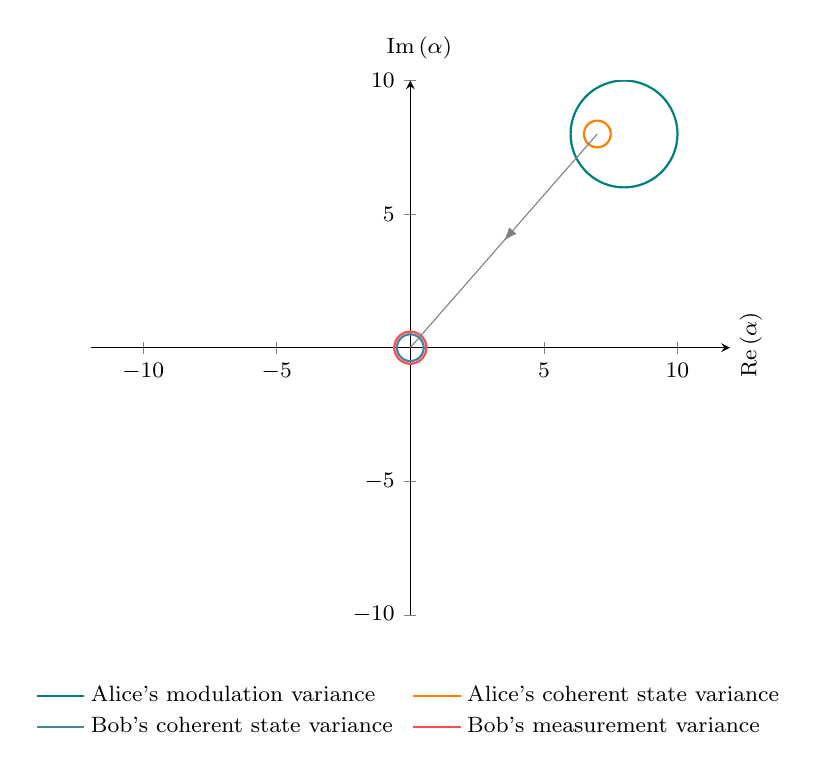
\begin{tikzpicture}[
		font=\fontsize{8}{9}\selectfont,
	]
		\begin{axis}[
			width=0.8\linewidth,
			axis lines=center,
			axis equal,
			no markers,
			cycle list name=exotic,
			xlabel={$\Re\left(\alpha\right)$},
			ylabel={$\Im\left(\alpha\right)$},
			xmin=-10,
			xmax=+10,
			ymin=-10,
			ymax=+10,
			domain=-180:180,
			samples=100,
			x label style={
				at={(ticklabel cs:1.0)},
				anchor=north,
				rotate=90,
				xshift=16,
			},
			y label style={
				at={(ticklabel cs:1.1)},
				xshift=12.0
			},
			legend style={
				at={(0.5,-0.25)},
				anchor=south,
				draw=none,
				/tikz/column 2/.style={
                	column sep=5pt,
	            },
			},
			legend cell align=left,
			legend columns=2,
		]
			\addplot+[thick]({8.0+2*cos(x)}, {8+2*sin(x)});
			\addlegendentry{Alice's modulation variance};
			\addplot+[thick]({7.0+0.5*cos(x)}, {8.0+0.5*sin(x)});
			\addlegendentry{Alice's coherent state variance};
			\addplot+[thick]({0.5*cos(x)}, {0.5*sin(x)});
			\addlegendentry{Bob's coherent state variance};
			\addplot+[thick]({0.6*cos(x)}, {0.6*sin(x)});
			\addlegendentry{Bob's measurement variance};
			
			\begin{scope}[
				decoration={
					markings,
					mark=at position 0.5 with {\arrow{Latex}},
				},
			]
				\draw[gray, postaction={decorate}] (axis cs:7,8) -- (axis cs:0,0);
			\end{scope}
		\end{axis}
	\end{tikzpicture}
\end{document}